\section{Methods}

% Describe the design process you plan to use and its tasks, how collaboration with stakeholders outside the course will be organised (societal organisation, researchers), any divisions of responsibilities, etc. Apply a participatory design methodology. The following headlines are used for organising the content of these different aspects. Remember that the methods and theories you choose are key to be able to answer your research questions!

We employ a participatory design process defined by iterative cycles of co-design, prototyping, and reflection~\cite{sanders2008evolving}. Collaborative tasks range from identifying learning goals to refining prototypes with stakeholders, including 10 to 12 year-old learners and educators. Stakeholders contribute domain knowledge, while our team manages prototyping, and ensures theoretical alignment.

\subsection{Analysis of the Use Situation}

% Analyse and describe a use scenario using theories presented in this course, in particular, Self-Determination Theory (needs and types of motivation), Self-Classification Theory, and Activity Theory (AT) (apply the following AT models: hierarchical model of activity, Engestr�m�s model, ZPD). Take as starting point the activity to be performed, the environment, the potential end users, and potential digital/physical material/instruments. The analysis forms the basis for the knowledge base and user models. Plan using the theories to prepare for what information and knowledge to obtain in meetings with stakeholders.

The use situation is situated within the mathematics classroom for students aged 10--12. While the subject (the student) aims to acquire mathematical reasoning skills (object), the community context is defined by heterogeneity, where student capabilities within a single class often span several grades. This disparity creates a conflict in the division of labor: a single teacher cannot simultaneously provide the individualized attention required to keep every student within their optimal Zone of Proximal Development (ZPD)~\cite{vygotsky1978mind}. Consequently, students often turn to the alternative avenues, such as standard AI chat-bots, to procure answers, rather than engaging in problem-solving.

\begin{figure}[ht]
    \centering
    \resizebox{0.9\textwidth}{!}{
        \begin{tikzpicture}[
            >={Stealth[length=3mm]},
            box/.style={
                    rectangle, rounded corners=4pt, draw, fill=blue!15,
                    minimum width=3.2cm, minimum height=1cm, align=center, font=\small
                },
            desc/.style={
                    font=\small, align=center
                },
            ]

            % Top
            \node[box] (instruments) {Instruments};

            % Middle
            \node[box, below left=2cm and 1cm of instruments] (subject) {Subject};
            \node[box, below right=2cm and 1cm of instruments] (object) {Object};

            % Bottom
            \node[box, below left=2cm and 1cm of subject] (rules) {Rules};
            \node[box, below right=2cm and 1cm of object] (division) {Division of\\Labor};
            \node[box] at ($(rules)!0.5!(division)$) (community) {Community};

            % Descriptions
            \node[desc, right=0.3cm of instruments] {Standard generative AI chatbots};
            \node[desc, left=0.3cm of subject] {Students aged 10--12};
            \node[desc, right=0.3cm of object] {Acquire mathematical\\reasoning skills};
            \node[desc, left=0.3cm of rules] {Curriculum standards,\\time constraints,\\classroom norms};
            \node[desc, below=0.2cm of community] {Mixed-ability classroom};
            \node[desc, right=0.3cm of division] {Single Teacher};

            % Arrows
            \draw[<->] (subject) -- (instruments);
            \draw[<->] (instruments) -- (object);
            \draw[<->] (subject) -- (object);

            \draw[<->] (subject) -- (rules);
            \draw[<->] (subject) -- (community);
            \draw[<->] (subject) -- (division);

            \draw[<->] (object) -- (rules);
            \draw[<->] (object) -- (community);
            \draw[<->] (object) -- node[right, font=\small\itshape, red!70!black] {Insufficient support within students' ZPD} (division);

            \draw[<->] (instruments) -- (community);

            \draw[<->] (rules) -- (community);
            \draw[<->] (community) -- node[below, font=\small\itshape, red!70!black, align=center] {Primary Contradiction} (division);

        \end{tikzpicture}
    }

    \caption{Engestr\"om's activity system of the current mathematics classroom.}
    \label{fig:activity_system}
\end{figure}

As illustrated in Figure \ref{fig:activity_system}, the primary systemic contradiction emerges between the division of labor (a single teacher) and the heterogeneous classroom community. This misalignment results in insufficient individualized activity within students' ZPD.

\subsection{Use Scenario}

% Provide a brief scenario for what your demonstrator will do in collaboration with a user.

The user, a learner, plays a card-based combat game as illustrated in Figure \ref{fig:gameplay_diagram} where each card is locked by a mathematical challenge. To unlock and play a card, the learner must solve the associated problem; incorrect answers result in a reduction of card power. The goal is to defeat an adversary and advance to a further stage. When stuck on a challenge, the learner can prompt an in-game agent for help. The agent does not provide the answer directly, but instead asks guiding questions to help the learner reason through the problem. Over the course of a session, the system adapts to the learner's strengths and weaknesses, tailoring both the difficulty of challenges and the guidance provided.

\begin{figure}[ht]
    \centering
    \resizebox{0.8\textwidth}{!}{
        \begin{tikzpicture}[
            >={Stealth[length=3mm]},
            startstop/.style={
                    circle, fill=black,
                },
            action/.style={
                    rectangle, rounded corners=4pt, draw, fill=blue!8,
                    minimum width=3.8cm, minimum height=1cm,
                    align=center, font=\small
                },
            decision/.style={
                    diamond, draw, fill=orange!15,
                    minimum width=2cm, minimum height=1.5cm,
                    align=center, aspect=2, font=\small
                },
            output/.style={
                    rectangle, rounded corners=4pt, draw=green!50!black, fill=green!8,
                    minimum width=3.8cm, minimum height=1cm,
                    align=center, font=\small
                },
            label/.style={
                    font=\scriptsize, fill=white, inner sep=1pt
                },
            ]

            % Main Flow
            \node[startstop] (start) {};
            \node[action, below=of start] (present) {Present Math Challenge};
            \node[action, below=of present] (attempt) {Student Submits Answer};
            \node[decision, below=3cm of attempt] (correct) {Correct?};

            % Help path
            \node[action, left=of attempt] (askhelp) {Request Help\\from Agent};
            \node[action, below=of askhelp] (guide) {Receive Guiding\\Question};

            % Incorrect
            \node[action, right=1.7cm of correct] (penalty) {Reduce Card\\Effect};

            % Correct
            \node[action, left=1.7cm of correct] (unlock) {Unlock Card};
            \node[action, below=of unlock] (play) {Play Card in Combat};
            \node[decision, below=of play] (repeat) {Play Another\\Card?};

            % End turn
            \node[action, right=of repeat] (damage) {Enemy Deals Damage};
            \node[decision, right=of damage] (alive) {Still Alive?};
            \node[output, above=of alive] (gameover) {Game Over};

            % Arrows

            % Main flow
            \draw[->] (start) -- (present);
            \draw[->] (present) -- (attempt);
            \draw[->] (attempt) -- (correct);

            % Help path
            \draw[->] (attempt) -- node[label, above] {Stuck} (askhelp);
            \draw[->] (askhelp) -- (guide);
            \draw[->] (guide.south) -- ++(0,-0.5) -| ([xshift=-0.5cm]attempt.south);

            % Incorrect path
            \draw[->] (correct) -- node[label, above] {No} (penalty);
            \draw[->] (penalty.east) -- ++(0.5,0) -| ([xshift=5.2cm]attempt.east) -- (attempt.east);

            % Correct path
            \draw[->] (correct) -- node[label, above] {Yes} (unlock);
            \draw[->] (unlock) -- (play);
            \draw[->] (play) -- (repeat);
            \draw[->] (repeat.west) -- ++(-0.5,0) -| node[pos=0.1, below] {Yes} ([xshift=-5.2cm]present.west) -- (present.west);

            % End turn
            \draw[->] (repeat) -- node[label, above] {No} (damage);
            \draw[->] (damage) -- (alive);
            \draw[->] (alive) -- node[label, left] {No} (gameover);
            \draw[->] (alive.east) -- ++(0.5,0) -| node[pos=0.1, below] {Yes} ([xshift=5.6cm]present.east) -- (present.east);

        \end{tikzpicture}
    }

    \caption{Activity diagram of the gameplay loop.}
    \label{fig:gameplay_diagram}
\end{figure}

\subsection{Procedure for the Participatory Design Process Involving Stakeholders}

% What stakeholders would be interesting to involve, which ones are available? What will be focused in meetings with stakeholders? How can you set up the meetings to most efficiently engage them in the design?

To ensure the system aligns with both pedagogical standards and the motivational needs of the target group, the design procedure organizes collaboration with a mathematics teacher and students aged 10--12. We conduct periodic check-ins with a teacher to define goals, mechanics, and inclusion needs, and final prototype evaluation with an undetermined amount of learners. During the evaluation, students are asked to critique the dialogue style, thereby allowing them to shape the \enquote{rewards} that support their sense of autonomy and competence~\cite{ryan2000self}. Each meeting produces prioritized action items to directly inform the next iteration.

\subsection{Anticipated Design Solution that will be Evaluated with Tentative Users}

% What will the anticipated design that will be evaluated with tentative users consist of based on what you know now? Will there be elements of behaviour change techniques? What kind of social behaviour?

The core of the design is a dynamic User Model operationalized within a RAG architecture, designed to function as a \enquote{More Knowledgeable Peer}. The system employs the \enquote{MiniGuide} strategy as a strict constraint on the RAG generation layer, thereby forcing the LLM to generate guiding questions that maintain the learner within their ZPD. Figure ~\ref{fig:data_flow_diagram} shows how these components interact at the system level.

\begin{figure}[ht]
    \centering
    \resizebox{0.8\textwidth}{!}{
        \begin{tikzpicture}[
            >={Stealth[length=3mm]},
            actor/.style={
                    ellipse, draw=blue!60, fill=blue!8,
                    minimum width=3cm, minimum height=1cm,
                    align=center, font=\small
                },
            process/.style={
                    rectangle, rounded corners=4pt, draw, fill=orange!10,
                    minimum width=3cm, minimum height=1cm,
                    align=center, font=\small
                },
            datastore/.style={
                    rectangle, draw, dashed, fill=purple!10, rounded corners=2pt,
                    minimum width=3cm, minimum height=1cm,
                    align=center, font=\small\itshape
                },
            output/.style={
                    rectangle, rounded corners=4pt, draw=green!50!black, fill=green!8,
                    minimum width=3cm, minimum height=1cm,
                    align=center, font=\small
                },
            label/.style={
                    font=\scriptsize, fill=white, inner sep=1pt
                },
            ]

            % Actor
            \node[actor] (learner) {Learner};

            % Row 1: Input processing
            \node[process, below=of learner] (intent) {Input Analysis};

            % Row 2: Two paths
            \node[process, below left=and 2.5cm of intent] (rag) {RAG Engine};
            \node[process, below right=and 2.5cm of intent] (difficulty) {Difficulty\\Matching};

            % Row 3: Generation / Reward
            \node[process, below=of rag] (llm) {MiniGuide LLM};
            \node[process, below=of difficulty] (reward) {Card Activation};

            % Row 4: Outputs
            \node[output, below=of llm] (question) {Guiding Question};
            \node[output, below=of reward] (gamestate) {Updated Game State};

            % Data stores
            \node[datastore, below=of intent] (curriculum) {Curriculum \&\\Heuristics KB};
            \node[datastore, below=of curriculum] (usermodel) {Dynamic User Model};

            % Arrows
            \draw[->] (learner) -- node[label, right] {Submit Answer / Ask for Help} (intent);
            \draw[->] (intent) -- node[label, above left] {Needs Help} (rag);
            \draw[->] (intent) -- node[label, above right] {Answer Submitted} (difficulty);

            % Left path: Help
            \draw[->] (rag) -- (llm);
            \draw[->] (llm) -- (question);
            \draw[->] (curriculum) -- (rag);

            % Right path: Game
            \draw[->] (difficulty) -- (reward);
            \draw[->] (reward) -- (gamestate);
            \draw[->] (curriculum) -- (difficulty);

            % Outputs back to learner
            \draw[->] (question.south) -- ++(0,-0.5) -| ([xshift=-7cm]learner.west) -- (learner.west);
            \draw[->] (gamestate.south) -- ++(0,-0.5) -| ([xshift=7cm]learner.east) -- (learner.east);

            % User model connections
            \draw[->, dashed] (usermodel) -- node[label, above] {ZPD} (llm);
            \draw[->, dashed] (usermodel) -- node[label, above left] {ZPD} (difficulty);
            \draw[->, dashed] (question.east) -- ++(1.5,0) node[label, above] {Update ZPD} -| ([xshift=-0.75cm]usermodel.south);
            \draw[->, dashed] (gamestate.west) -- ++(-1.5,0) node[label, above] {Update ZPD} -| ([xshift=0.75cm]usermodel.south);

        \end{tikzpicture}
    }

    \caption{Data flow diagram of the system architecture. Solid arrows indicate the primary data flow; dashed arrows indicate reads from and writes to the Dynamic User Model.}
    \label{fig:data_flow_diagram}
\end{figure}


\subsubsection{Game Design}

\begin{figure}[ht]
    \centering
    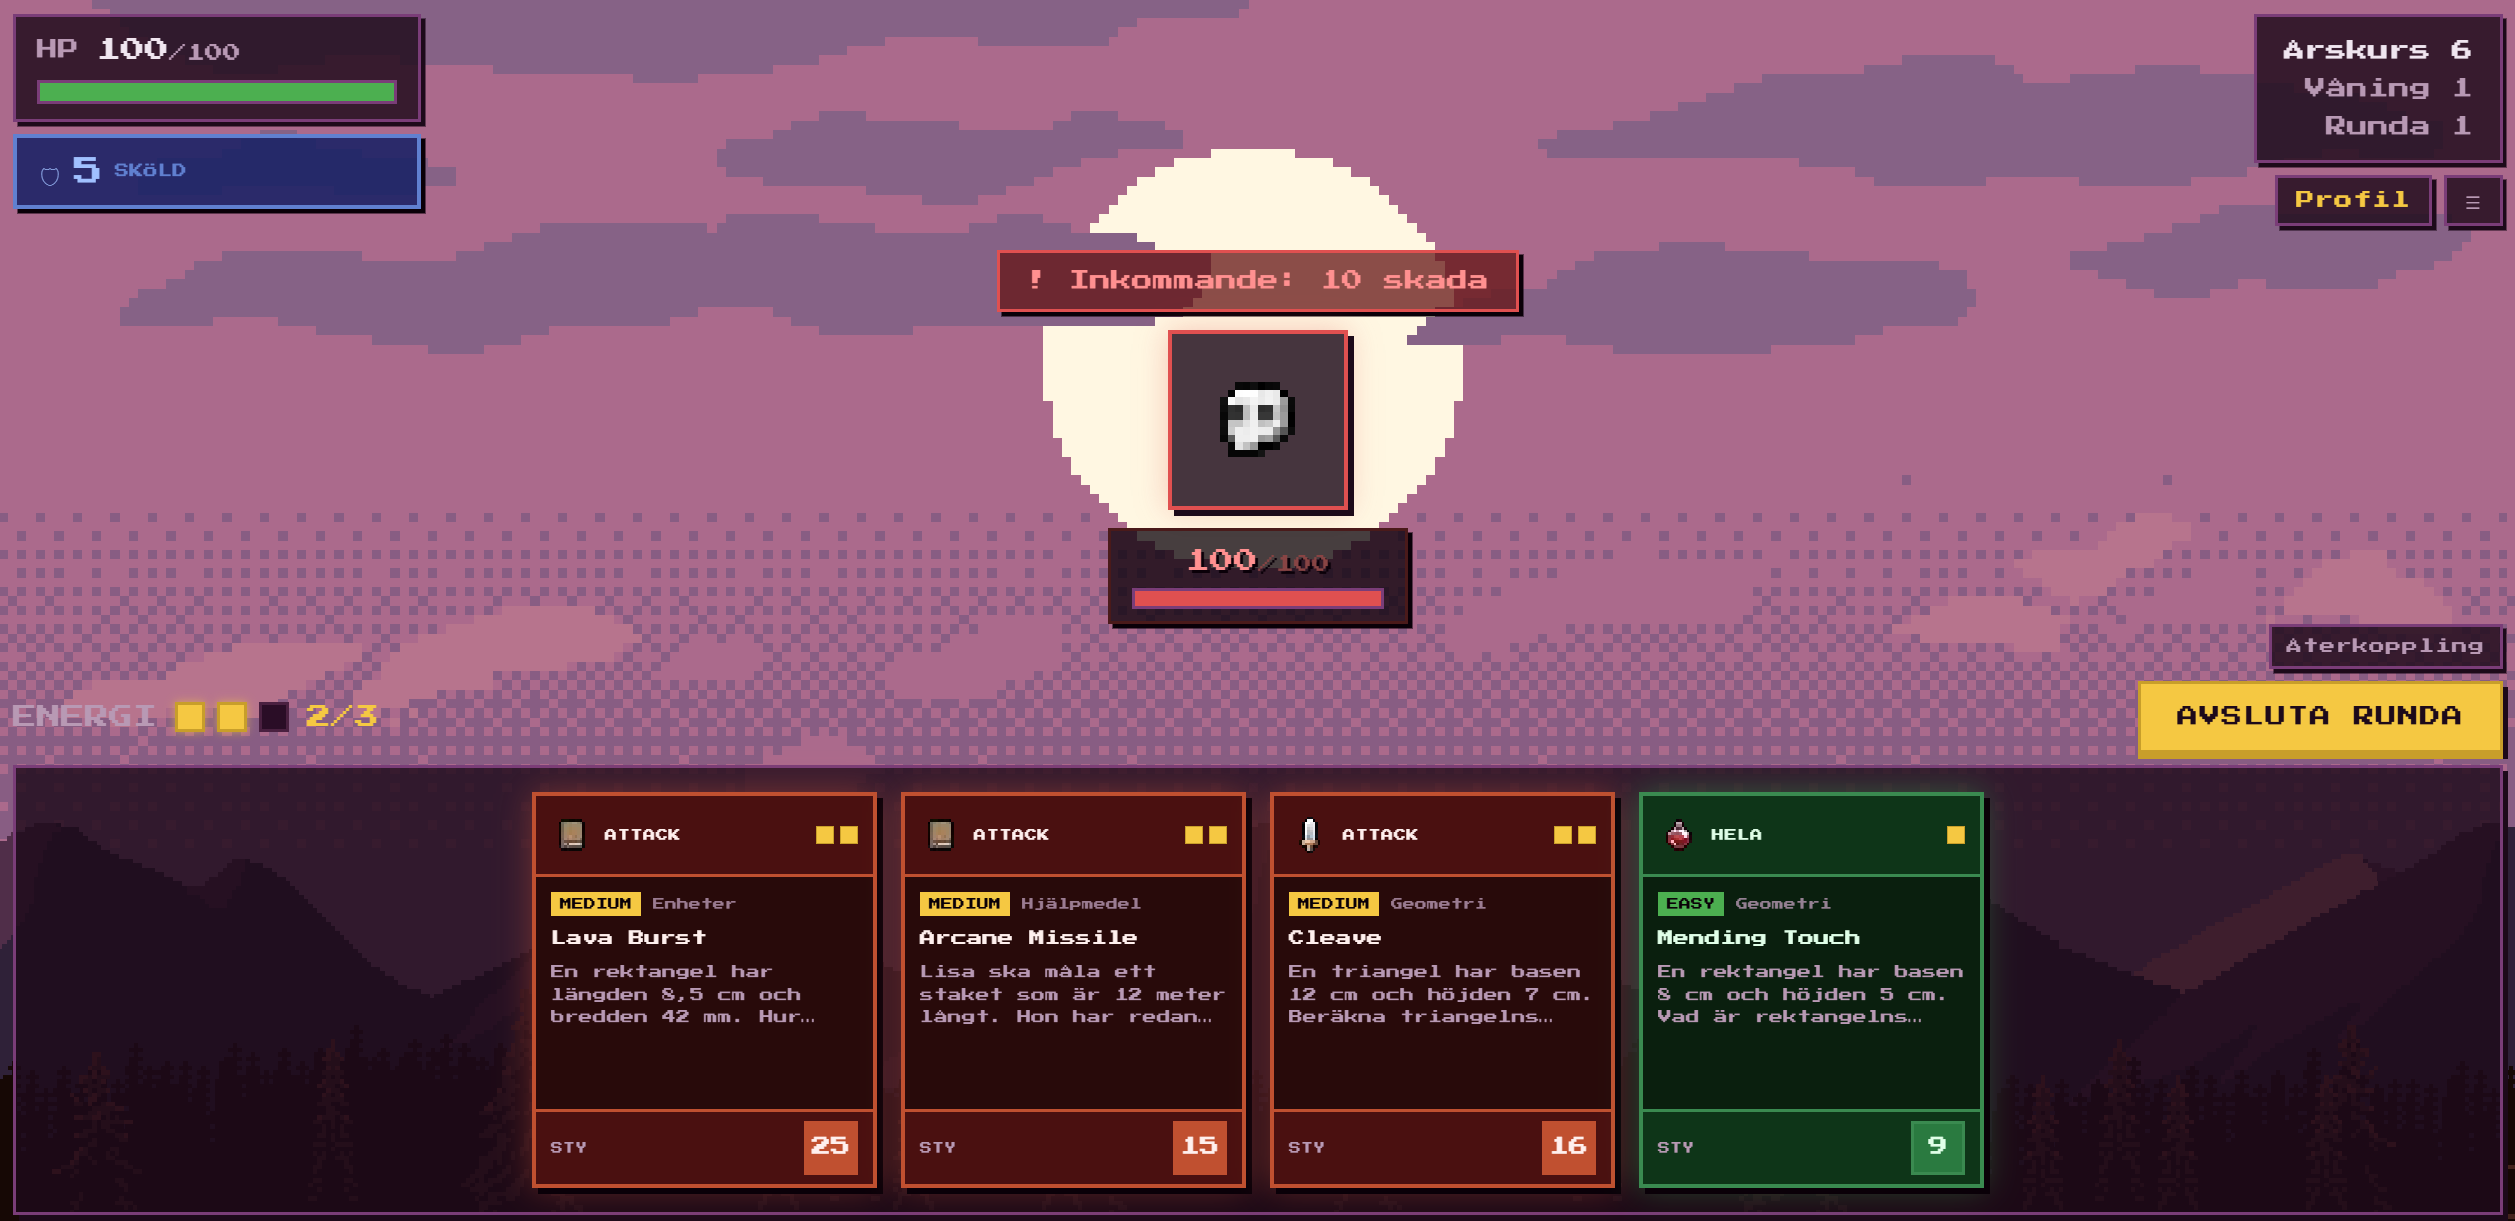
\includegraphics[width=0.8\textwidth]{../images/game_screen.png}
    \caption{The battle screen after a single turn. In the top right we see the players health and active shield. Centered on the screen is the enemy display, showing their health and damage that will be dealt next turn. Cards and their type, strength, energy cost, as well as topic and difficulty of the associated math challenge are displayed in the bottom.}
    \label{fig:game_screen}
\end{figure}

The learner plays a turn-based card combat game inspired by the roguelike deck-building genre. The player is presented with a hand of cards, each displaying its power value and associated challenge difficulty (Figure~\ref{fig:game_screen}). Each card in the player's hand is locked behind a mathematical challenge matched to their current ability level. To play a card, the learner must correctly solve the associated problem. The goal is to defeat an adversary and advance to the next stage, creating a gameplay loop where mathematical reasoning is the core mechanic rather than an interruption.

Cards vary in power, and stronger cards are gated by harder problems. This coupling serves a dual purpose: it motivates learners to attempt more difficult challenges for strategic advantage, and it naturally prevents progress without genuine mathematical engagement. Crucially, incorrect answers carry an in-game consequence in the form of card power reduction, mirroring the stakes of an actual game combat encounter. This mechanic discourages random guessing, ensuring that learners engage thoughtfully with each problem rather than treating the math as a low-cost obstacle to click through~\cite{xu2023exploring}.

\subsubsection{Scaffolding Through the \enquote{MiniGuide} Strategy}

When a learner is stuck on a challenge, they can request help from an in-game agent (Figure~\ref{fig:task_screen}). Rather than providing the answer, the agent follows the \enquote{MiniGuide} strategy: it first diagnoses the learner's current state using the User Model, then retrieves relevant curricular content from a knowledge base via RAG, and finally generates a guiding question designed to nudge the learner toward the solution. This preserves the learner's agency and keeps them actively reasoning.

\begin{figure}[ht]
    \centering
    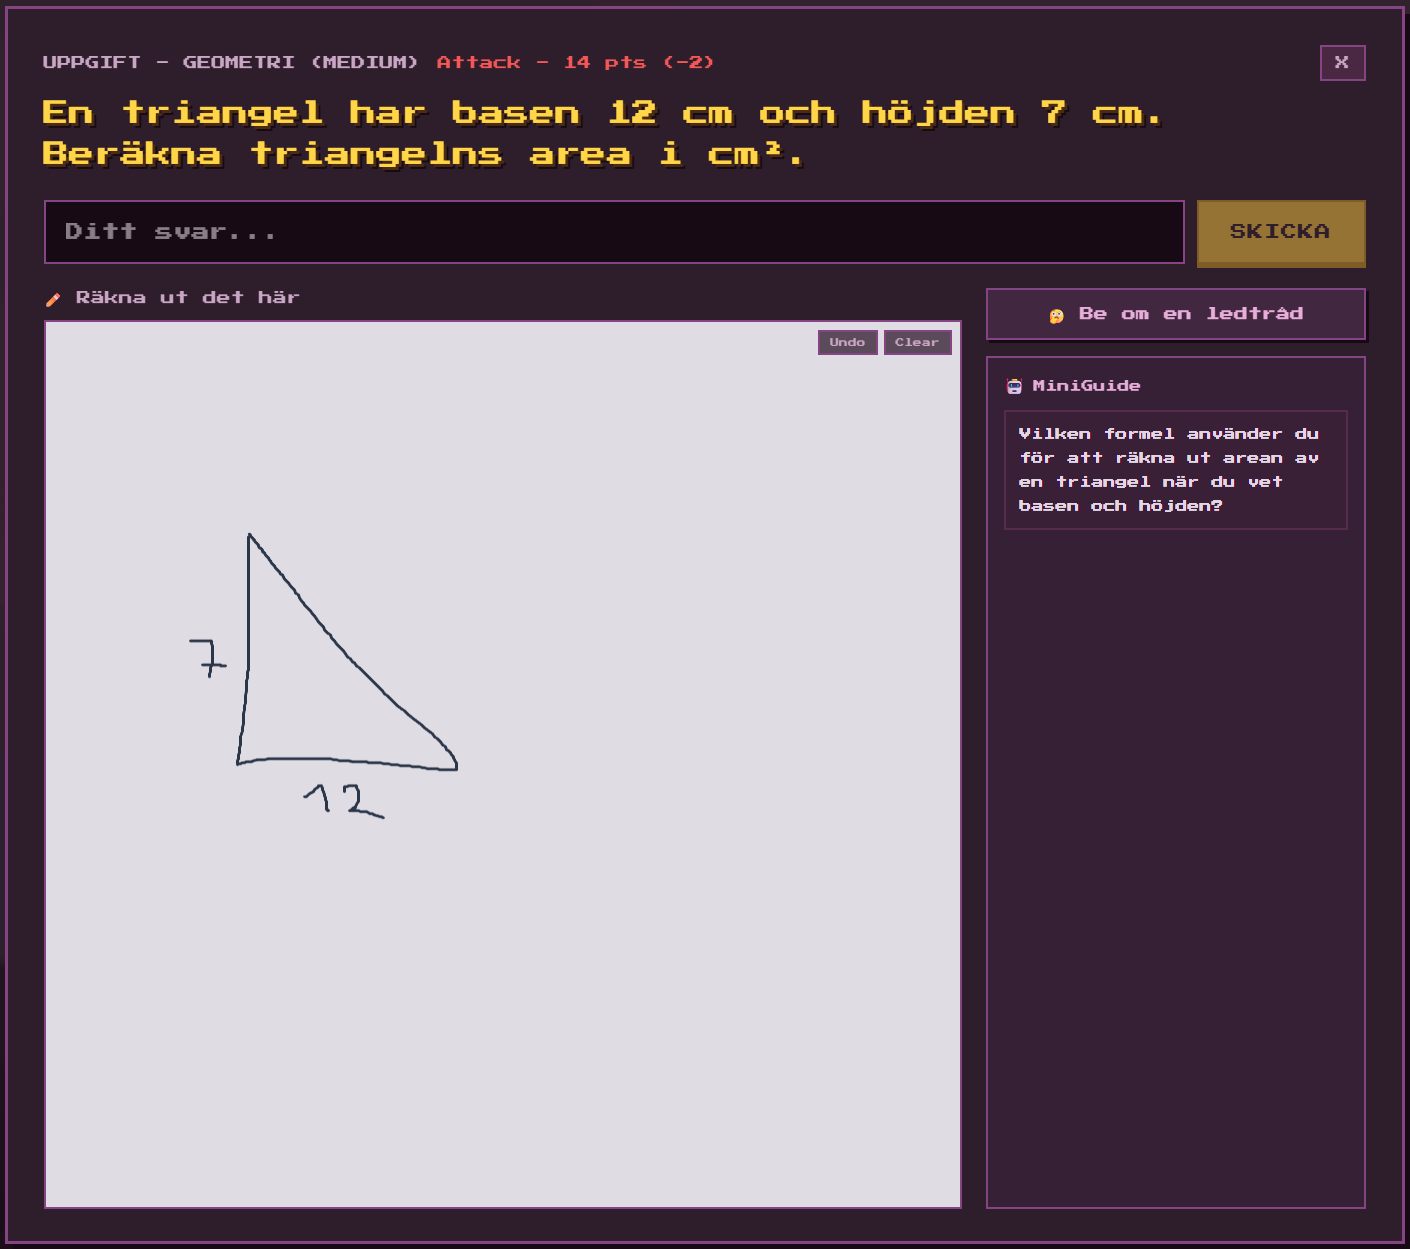
\includegraphics[width=0.8\textwidth]{../images/task_screen.png}
    \caption{The task screen for an easy \enquote{Tid \& Datum} math task, where the answer has been submitted, and the user has requested a hint. The player is presented with the question, a field for entering the answer, a whiteboard for sketching out solutions, and a button for getting a hint with the list of past hints below.}
    \label{fig:task_screen}
\end{figure}

The strict constraint on the generation layer aims to prevent the LLM from producing direct answers. Instead, its output is limited to diagnostic questions, hints, and prompts for reflection — functioning as a peer who helps the learner think, not one who thinks for them.

\subsubsection{Dynamic User Model}

Throughout a learning session, the system builds and refines a User Model that captures the learner's current mastery across mathematical topics, common error patterns, and help-seeking behavior. This model informs both the difficulty of challenges presented and the type of guidance the agent provides. For example, a learner who consistently struggles with fractions will receive challenges and guidance tailored to that gap, while a learner who frequently requests hints without attempting a solution first may receive prompts that encourage independent effort before offering guidance.

In practice, the system tracks correct and incorrect answer attempts and hint requests per difficulty, aggregated by topic. The content of the user model is presented in the user interface as the \enquote{Elevprofil} (Figure~\ref{fig:profile_screen}). When generating new tasks or guiding questions, these metrics are summarized using simple threshold based rules into a learner profile, as shown in Figure ~\ref{fig:user_model_diagram}, identifying strengths, weaknesses, and behavioral patterns, which is then included in the RAG context for subsequent interactions. This means the agent's responses become increasingly personalized over the course of a session, allowing the system to adapt both game difficulty and pedagogical approach to keep the learner within their ZPD.

\begin{figure}[ht]
    \centering
    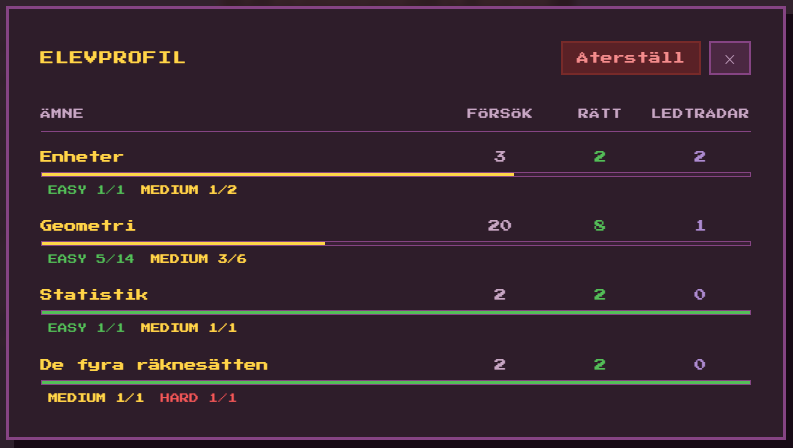
\includegraphics[width=0.8\textwidth]{../images/profile_screen.png}
    \caption{The user model (here called the student profile). The number of answer attempts, correct answers and number of hints received are displayed, grouped by topic.}
    \label{fig:profile_screen}
\end{figure}

\begin{figure}[ht]
    \centering
    \resizebox{0.8\textwidth}{!}{
        \begin{tikzpicture}[
            >={Stealth[length=3mm]},
            box/.style={
                    rectangle, rounded corners=3pt, draw, fill=blue!8,
                    minimum width=3cm, minimum height=1cm,
                    align=center, font=\small
                },
            data/.style={
                    rectangle, rounded corners=3pt, draw, dashed, fill=purple!8,
                    minimum width=3cm, minimum height=1cm,
                    align=center, font=\small\itshape
                },
            llmbox/.style={
                    rectangle, rounded corners=3pt, draw, fill=orange!12,
                    minimum width=3cm, minimum height=1cm,
                    align=center, font=\small
                },
            groupbox/.style={
                    rectangle, rounded corners=5pt, draw=gray!70, dashed,
                    inner sep=12pt
                },
            grouplabel/.style={
                    font=\small\bfseries, text=gray!70
                },
            label/.style={
                    font=\scriptsize, fill=white, inner sep=1pt
                },
            ]

            % Student interactions
            \node[box] (answer) {Answer Attempts};
            \node[box, right=of answer] (topics) {Topic Tags};
            \node[box, right=of topics] (hints) {Hint Requests};

            \node[groupbox, fit=(answer)(topics)(hints)] (metrics) {};
            \node[grouplabel, above=0pt of metrics.north] {Session Metrics};

            % LLM summarization
            \node[llmbox, below=of metrics] (llm) {LLM Summarization};

            % Output
            \node[box, below=of llm] (rag) {RAG Context};

            % Consumers
            \node[box, below left=of rag] (tasks) {Task\\Generation};
            \node[box, below right=of rag] (guidance) {Guidance\\Generation};

            % Arrows
            \draw[->] (metrics) -- (llm);
            \draw[->] (llm) -- (rag);
            \draw[->] (rag) -- (tasks);
            \draw[->] (rag) -- (guidance);

            % Feedback loop
            \draw[->, dashed, gray] (tasks.west) -- ++(-1,0) |-  (answer.west);
            \draw[->, dashed, gray] (guidance.east) -- ++(1,0) |-  (hints.east);

        \end{tikzpicture}
    }

    \caption{User Model creation process.}
    \label{fig:user_model_diagram}
\end{figure}

\subsubsection{Determining the Zone of Proximal Development}

The system approximates each learner's Zone of Proximal Development by classifying problem interactions into three categories based on the level of assistance required.

\begin{description}

    \item [Below:] Problems that the learner solves correctly without requesting any hints, these represent mastered material.\\$\left[Accuracy \geq 70\% \; \& \; hints = 0\right]$

    \item [Above:] Problems where the learner fails to arrive at the correct answer despite available assistance, these are beyond the learner's current reach.\\$\left[Accuracy < 40\% \; \& \; hints \geq 1\right]$

    \item [Within:] Problems that the learner solves correctly after receiving one or more guiding questions from the agent, these are the problems where scaffolding is most effective and where learning is most likely to occur.

\end{description}

This classification, summarized in Figure~\ref{fig:zpd_diagram}, is tracked per topic and accumulated over a session in the form of the user model.

\begin{figure}[ht]
    \centering
    \resizebox{0.8\textwidth}{!}{
        \begin{tikzpicture}[
            >={Stealth[length=3mm]},
            zone/.style={
                    rectangle, rounded corners=5pt, draw,
                    minimum width=9cm, minimum height=1.4cm,
                    align=center, font=\small
                },
            zlabel/.style={
                    font=\small\bfseries, align=right, text width=3cm
                },
            indicator/.style={
                    font=\small, align=left, text width=5.5cm
                },
            ]

            % Zones (stacked bottom to top)
            \node[zone, fill=green!15, draw=green!50!black] (below) {};
            \node[zone, fill=yellow!20, draw=yellow!60!black, above=2pt of below] (within) {};
            \node[zone, fill=red!12, draw=red!50!black, above=2pt of within] (above) {};

            % Zone labels (left side)
            \node[zlabel, left=0.1cm of above] {Above ZPD};
            \node[zlabel, left=0.1cm of within] {Within ZPD};
            \node[zlabel, left=0.1cm of below] {Below ZPD};

            % Indicators (inside zones)
            \node[indicator] at (above.center) {Incorrect despite assistance\\$\rightarrow$ Too difficult, reduce difficulty};
            \node[indicator] at (within.center) {Correct after guiding questions\\$\rightarrow$ Optimal learning zone, maintain};
            \node[indicator] at (below.center) {Correct without hints\\$\rightarrow$ Already mastered, increase difficulty};
        \end{tikzpicture}
    }

    \caption{Classification of problem interactions into ZPD regions.}
    \label{fig:zpd_diagram}
\end{figure}

\subsubsection{Gamification and Motivation}

The game structure is designed to align with Self-Determination Theory~\cite{ryan2000self} by supporting autonomy (choosing which cards to attempt), competence (solving challenges at an appropriate difficulty), and relatedness (interacting with the in-game agent as a supportive peer). Because card power is tied to problem difficulty relative to the learner's level, both high-performing and struggling learners face meaningful challenges — avoiding boredom for advanced students and reducing frustration for those who need more support.

Importantly, progress in the game is closely tied to demonstrated mathematical reasoning, and not surpassable game mechanics or repetition. This transforms the friction of learning into a core part of the game loop rather than an obstacle to it.


\subsection{Material and software}

% List the software that you would like to use and other material. Other material can be publicly available data sets, ontologies, etc. Available robots are the Furhat robot, and a NAO robot.

The prototype adopts a decoupled client-server web architecture to enable rapid prototyping and broad accessibility on standard school devices without requiring software installation. The frontend is developed using Next.js, a modern web framework built upon React, to manage the interactive gamified interface. Server-side logic is handled through a Python FastAPI backend, which orchestrates the RAG pipeline, game logic, and user modeling components.

A multimodal Large Language Model is required to process handwritten mathematical input from the canvas interface. The prototype uses Anthropic's Claude Sonnet 4.6 for both handwriting recognition and guided response generation, but the long-term architecture anticipates replacing the third party model with a self-hosted, or EU-based model to better align with data privacy requirements for use in schools.

The RAG framework is connected to a curriculum-aligned knowledge base indexed within a vector database. For mathematical content, the system draws on Matteboken.se, a free and comprehensive digital mathematics resource provided by the Swedish nonprofit Mattecentrum. The platform covers the full Swedish curriculum for mellanstadiet (grades 4--6), including arithmetic operations, geometry, units of measurement, statistics, and time, providing a structured and openly accessible content base for the retrieval corpus.

\subsubsection{LLM prompting and output stability}

The system communicates with the LLM using three system prompts, each strictly scoped to a single responsibility: task generation, guidance generation, and topic \& difficulty selection. All prompts follow the same structure: a role definition, explicit behavioral constraints, and a required JSON output schema.

To ensure stable and parseable output, all prompts require the LLM to respond with a JSON object matching a predefined schema, with no additional text, markdown formatting, or preamble. This allows the backend to parse responses without relying on text extraction. When the response does not conform to the expected schema, the system rejects it and retries the request rather than passing malformed output to the student.

\subsection{Evaluation setup}

% What will be focused in meetings with tentative users? What will be evaluated? What participants?

The evaluation adopts an exploratory, qualitative approach. It consists of two sessions with distinct participant groups.

The first session involves a teacher acting as the domain expert during which we focus on evaluating the RAG system's generation layer: whether the guiding questions produced by the \enquote{MiniGuide} strategy are pedagogically sound, and question content and difficulty is appropriate for the target grade. The teacher interacts with the system and provides feedback on the state of the prototype.

During the second session, the system is distributed to an undetermined number of school students aged 10--12 (2-3 classrooms, upward of 20 students). This session focuses on usability and engagement rather than learning outcomes, as a single session is insufficient to measure knowledge gains. Students are presented with a simple questionnaire to capture the students' disposition towards the system. The questionnaire is built into the system (Figure~\ref{fig:questionnaire_screen}) and consists of the following questions:

\begin{itemize}
    \item \textbf{Q1:} How would you rate your math skill level? (1--5)\\\enquote{Hur bedömer du din matematikförmåga?}
    \item \textbf{Q2:} How difficult do you find the math tasks? (1--5)\\\enquote{Hur svåra tycker du att matematikuppgifterna är?}
    \item \textbf{Q3:} How helpful are the hints when you use them? (1--5)\\\enquote{Hur hjälpsamma är ledtrådarna när du använder dem?}
    \item \textbf{Q4:} How likely are you to play this in your spare time? (1--5)\\\enquote{Hur troligt är det att du spelar det här på fritiden?}
    \item \textbf{Q5:} How stressed do you feel while playing? (1--5)\\\enquote{Hur stressad känner du dig när du spelar?}
    \item Gender (Male, Female, Other, Prefer not to say)
    \item Age
\end{itemize}

\begin{figure}[ht]
    \centering
    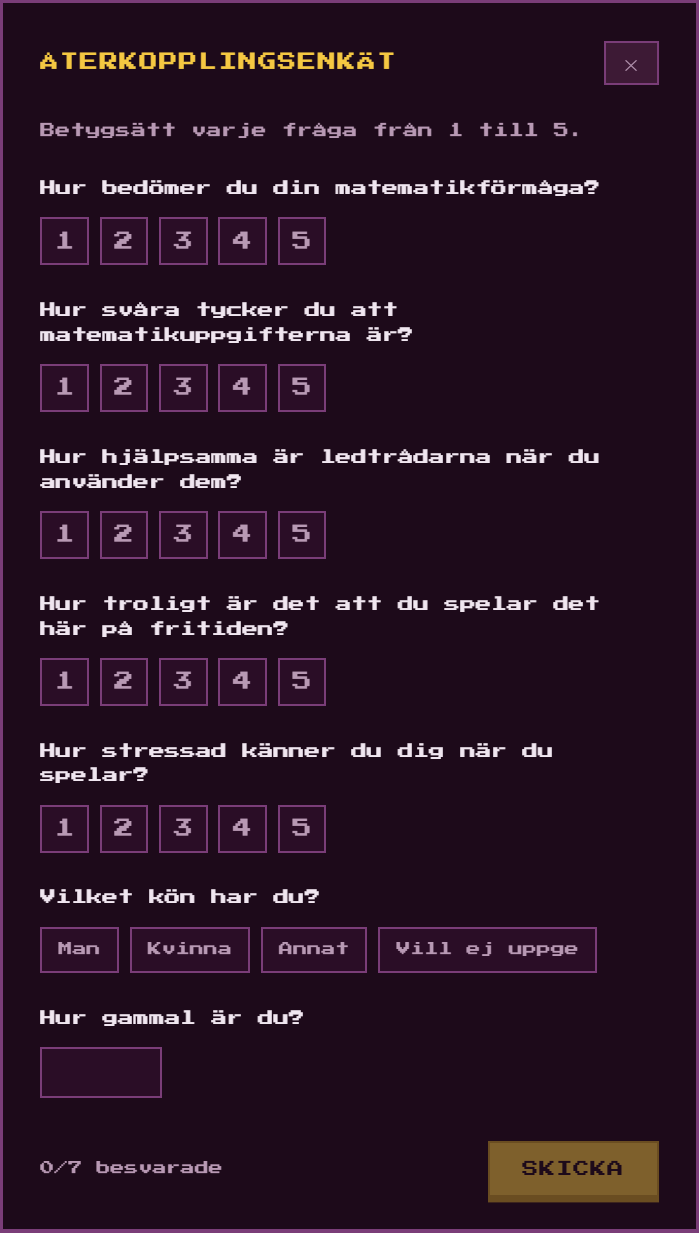
\includegraphics[width=0.5\textwidth]{../images/questionnaire_screen.png}
    \caption{Questionnaire integrated into the system.}
    \label{fig:questionnaire_screen}
\end{figure}